%!TEX TS-program = xelatex
\documentclass[12pt, a4paper, oneside]{article}

\usepackage{amsmath,amsfonts,amssymb,amsthm,mathtools}  % пакеты для математики

\usepackage[utf8]{inputenc} % задание utf8 кодировки исходного tex файла
\usepackage[british,russian]{babel} % выбор языка для документа

\usepackage{fontspec}         % пакет для подгрузки шрифтов
\setmainfont{Helvetica}   % задаёт основной шрифт документа

\usepackage{unicode-math}     % пакет для установки математического шрифта
\setmathfont{Neo Euler}      % шрифт для математики
% \setmathfont[math-style=ISO]{Asana Math}
% Можно делать смену начертания с помощью разных стилей

% Конкретный символ из конкретного шрифта
% \setmathfont[range=\int]{Neo Euler}

%%%%%%%%%% Работа с картинками %%%%%%%%%
\usepackage{graphicx}                  % Для вставки рисунков
\usepackage{graphics}
\graphicspath{{images/}{pictures/}}    % можно указать папки с картинками
\usepackage{wrapfig}                   % Обтекание рисунков и таблиц текстом

%%%%%%%%%%%%%%%%%%%%%%%% Графики и рисование %%%%%%%%%%%%%%%%%%%%%%%%%%%%%%%%%
\usepackage{tikz, pgfplots}  % язык для рисования графики из latex'a

%%%%%%%%%% Гиперссылки %%%%%%%%%%
\usepackage{xcolor}              % разные цвета

\usepackage{hyperref}
\hypersetup{
	unicode=true,           % позволяет использовать юникодные символы
	colorlinks=true,       	% true - цветные ссылки, false - ссылки в рамках
	urlcolor=blue,          % цвет ссылки на url
	linkcolor=red,          % внутренние ссылки
	citecolor=green,        % на библиографию
	pdfnewwindow=true,      % при щелчке в pdf на ссылку откроется новый pdf
	breaklinks              % если ссылка не умещается в одну строку, разбивать ли ее на две части?
}


\usepackage{todonotes} % для вставки в документ заметок о том, что осталось сделать
% \todo{Здесь надо коэффициенты исправить}
% \missingfigure{Здесь будет Последний день Помпеи}
% \listoftodos --- печатает все поставленные \todo'шки

\usepackage[paper=a4paper, top=20mm, bottom=15mm,left=20mm,right=15mm]{geometry}
\usepackage{indentfirst}       % установка отступа в первом абзаце главы

\usepackage{setspace}
\setstretch{1.15}  % Межстрочный интервал
\setlength{\parskip}{4mm}   % Расстояние между абзацами
% Разные длины в латехе https://en.wikibooks.org/wiki/LaTeX/Lengths


\usepackage{xcolor} % Enabling mixing colors and color's call by 'svgnames'

\definecolor{MyColor1}{rgb}{0.2,0.4,0.6} %mix personal color
\newcommand{\textb}{\color{Black} \usefont{OT1}{lmss}{m}{n}}
\newcommand{\blue}{\color{MyColor1} \usefont{OT1}{lmss}{m}{n}}
\newcommand{\blueb}{\color{MyColor1} \usefont{OT1}{lmss}{b}{n}}
\newcommand{\red}{\color{LightCoral} \usefont{OT1}{lmss}{m}{n}}
\newcommand{\green}{\color{Turquoise} \usefont{OT1}{lmss}{m}{n}}

\usepackage{titlesec}
\usepackage{sectsty}
%%%%%%%%%%%%%%%%%%%%%%%%
%set section/subsections HEADINGS font and color
\sectionfont{\color{MyColor1}}  % sets colour of sections
\subsectionfont{\color{MyColor1}}  % sets colour of sections

%set section enumerator to arabic number (see footnotes markings alternatives)
\renewcommand\thesection{\arabic{section}.} %define sections numbering
\renewcommand\thesubsection{\thesection\arabic{subsection}} %subsec.num.

%define new section style
\newcommand{\mysection}{
	\titleformat{\section} [runin] {\usefont{OT1}{lmss}{b}{n}\color{MyColor1}} 
	{\thesection} {3pt} {} } 


%	CAPTIONS
\usepackage{caption}
\usepackage{subcaption}
%%%%%%%%%%%%%%%%%%%%%%%%
\captionsetup[figure]{labelfont={color=Turquoise}}

\pagestyle{empty}

\begin{document}

\section*{Семинар 2-3:  сегментация клиентов и кластеризация}

\todo[inline]{Задача на tf_idf}

\todo[inline]{Напомнить про OHE и как предобрабатывать фичи}


\subsection*{Задача 1 }

Тут будет задача про расстояния. В первом пункте между несколькими точками эти расстояния надо будет посчитать. Во втором пункте будут рисунки и вопросы какое расстояние лучше использовать. 

Идеи рисунков: две точки в поле --- евклидово, между небоскребами по улицам --- манхеттенское и тп. 


\subsection*{Задача 2}

На картинках ниже синими точками отмечены наблюдения. Красными точками отмечены стартовые центроиды для алгоритма $K$-means. 

\begin{minipage}[t]{0.45\textwidth}
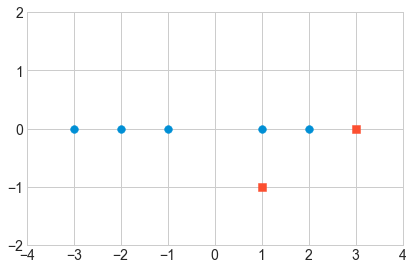
\includegraphics[scale=0.5]{knn1.png}
\end{minipage}
\hfill
\begin{minipage}[t]{0.45\textwidth}
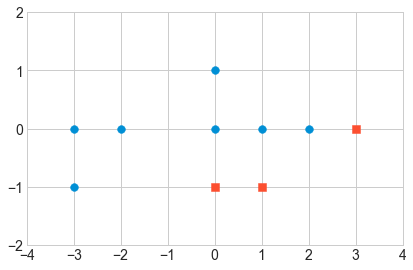
\includegraphics[scale=0.5]{knn2.png}
\end{minipage}

Кластеризуйте данные на первой картинке на два кластера, на второй картинке на три кластера. Сколько итераций понадобилось сделать до полной сходимости алгоритма? Сколько объектов вошли в каждый из кластеров? 

\begin{enumerate}
	\item[а)] Используйте для кластеризации Евклидово расстояние.
	\item[б)] Используйте для кластеризации Манхеттенское расстояние.
	\item[в)] В этой задачке мы сами предложили вам для кластеризации начальные точки (красные квадраты). На практике начальное приближение центроидов обычно генерирует компьютер.  Изменится ли разбиение на кластеры, если изменить стартовые точки?
\end{enumerate}


\subsection*{Задача 3 }

Начальник Аристарх был в командировке. Там он услышал про иерархическую агломеративную кластеризацию. По приезду, находясь в состоянии восторга, он записал в свой блокнот следующие четыре наблюдения:

\begin{center}
\begin{tabular}{c|c}
	\hline
	$x$ & $z$ \\
	\hline
	8 & 6   \\
	6 & 10 \\
	2 & 4   \\
	4 & 2   \\
\end{tabular}
\end{center}

После он отдал блокнот маркетологу Савелию. Аристарх хочет, чтобы Савелий провел агломеративную иерархическую кластеризацию.  На совещаний было решено использовать в качестве расстояния между объектами обычное Евклидово расстояние. Расстояние между кластерами решено определять по принципу дальнего соседа. Помогите Савелию с агломеративной иерархической кластеризацией. И не забудьте нарисовать дендрограмму. Начальники любят красивые картинки. 

\section*{Ещё задачи!}


\subsection*{Задача 4} 

\begin{center}
	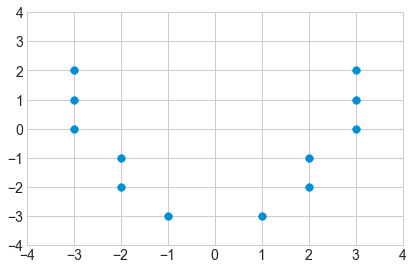
\includegraphics[scale=0.7]{knn_3.png}
\end{center}

\begin{enumerate}
	\item Примените метод $K$-means с $K=2$, $K=3$, $K=4$ и $K=5$. Начальные точки каждый раз выбирайте случайно.  Для всех ли начальных точек кластеризация каждый раз будет выдавать один и тот же результат? 
	\item Примените метод агломеративной иерархической кластеризации. Нарисуйте дендрограмму. Руководствуясь дендрограммой выберете оптимальное количество кластеров. Обоснуйте свой выбор.
	\item Правда ли, что для всех рассмотренных $K$ оба метода разбивают выборку на одинаковые кластеры?  Всегда ли так происходит? Приведите контр-пример. 
	
	\item Сюда вопрос про выбор оптимального k по межкластерному расстоянию и силуэту.
	
\end{enumerate}


\subsection*{Задача 5} 

Обозначьте расположение центроидов и границ кластеров после применения метода K-means c $K=2$ на следущих данных: 

\begin{center}
 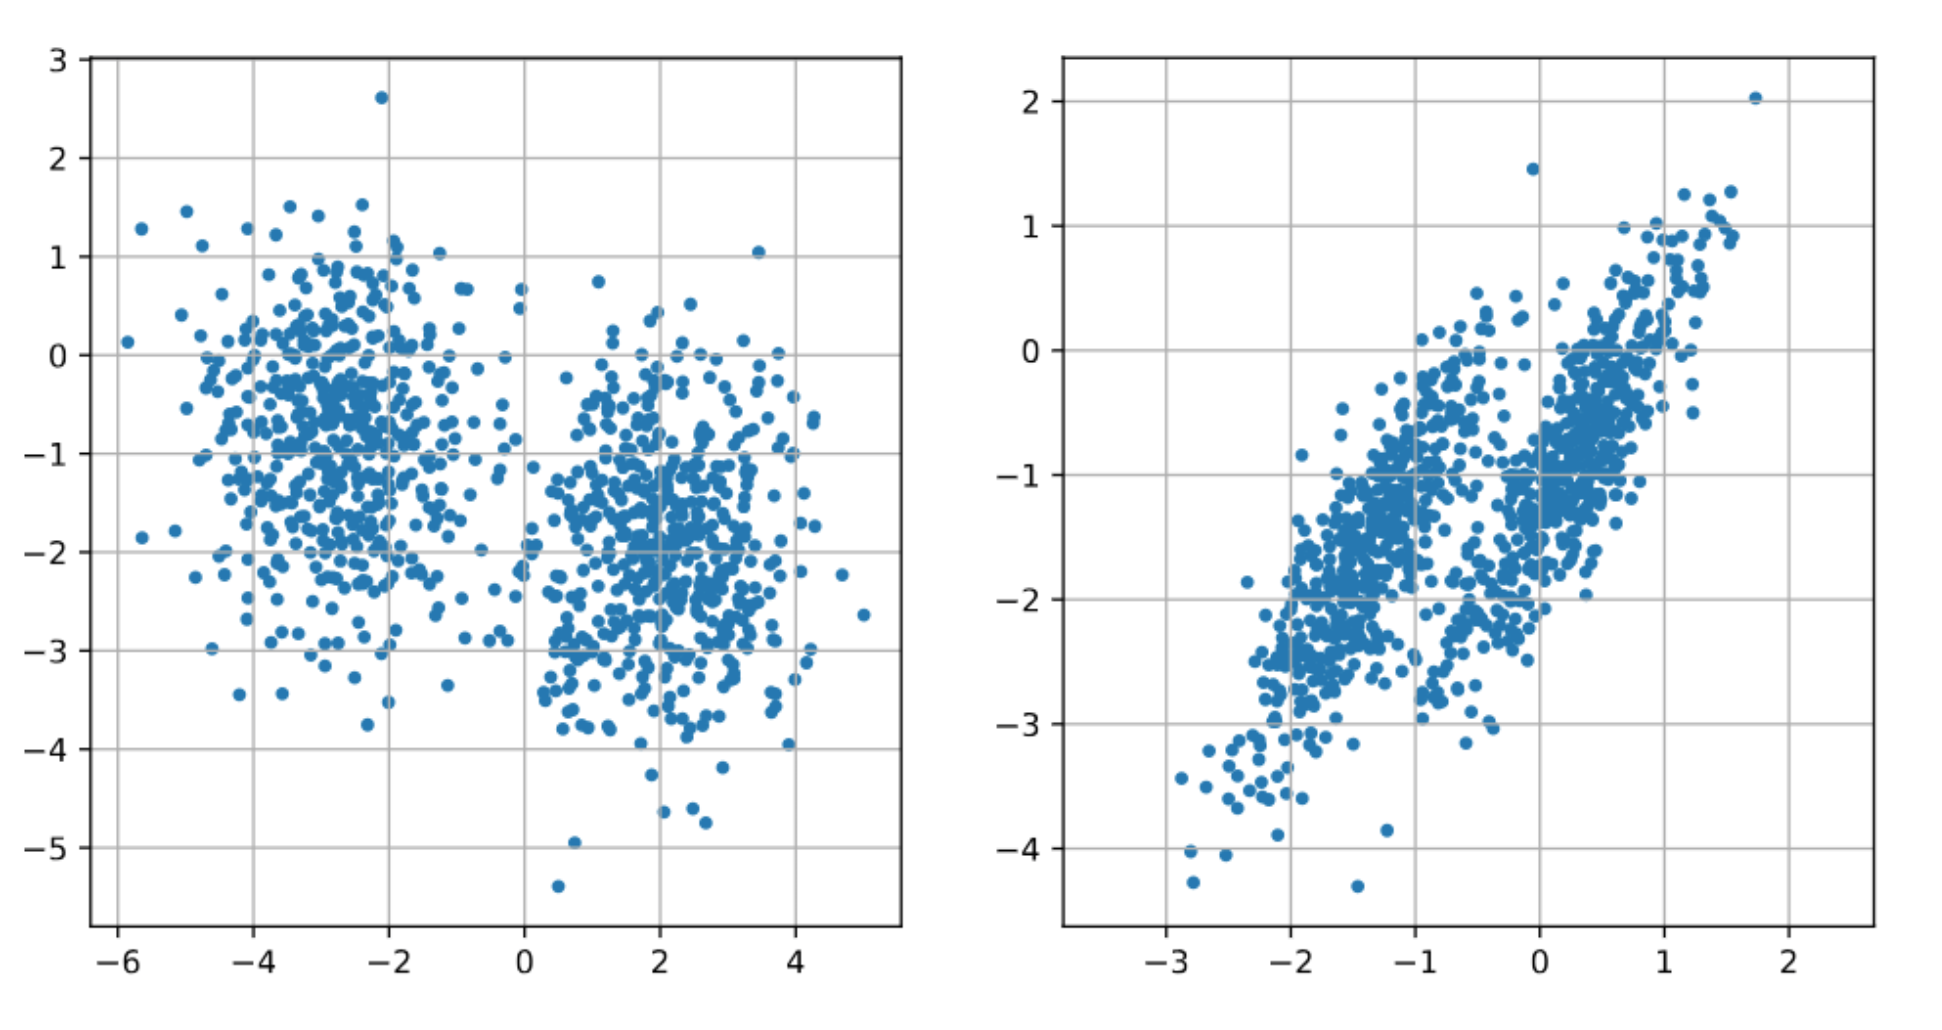
\includegraphics[scale=0.2]{clouds.png}
\end{center}

\begin{center}
	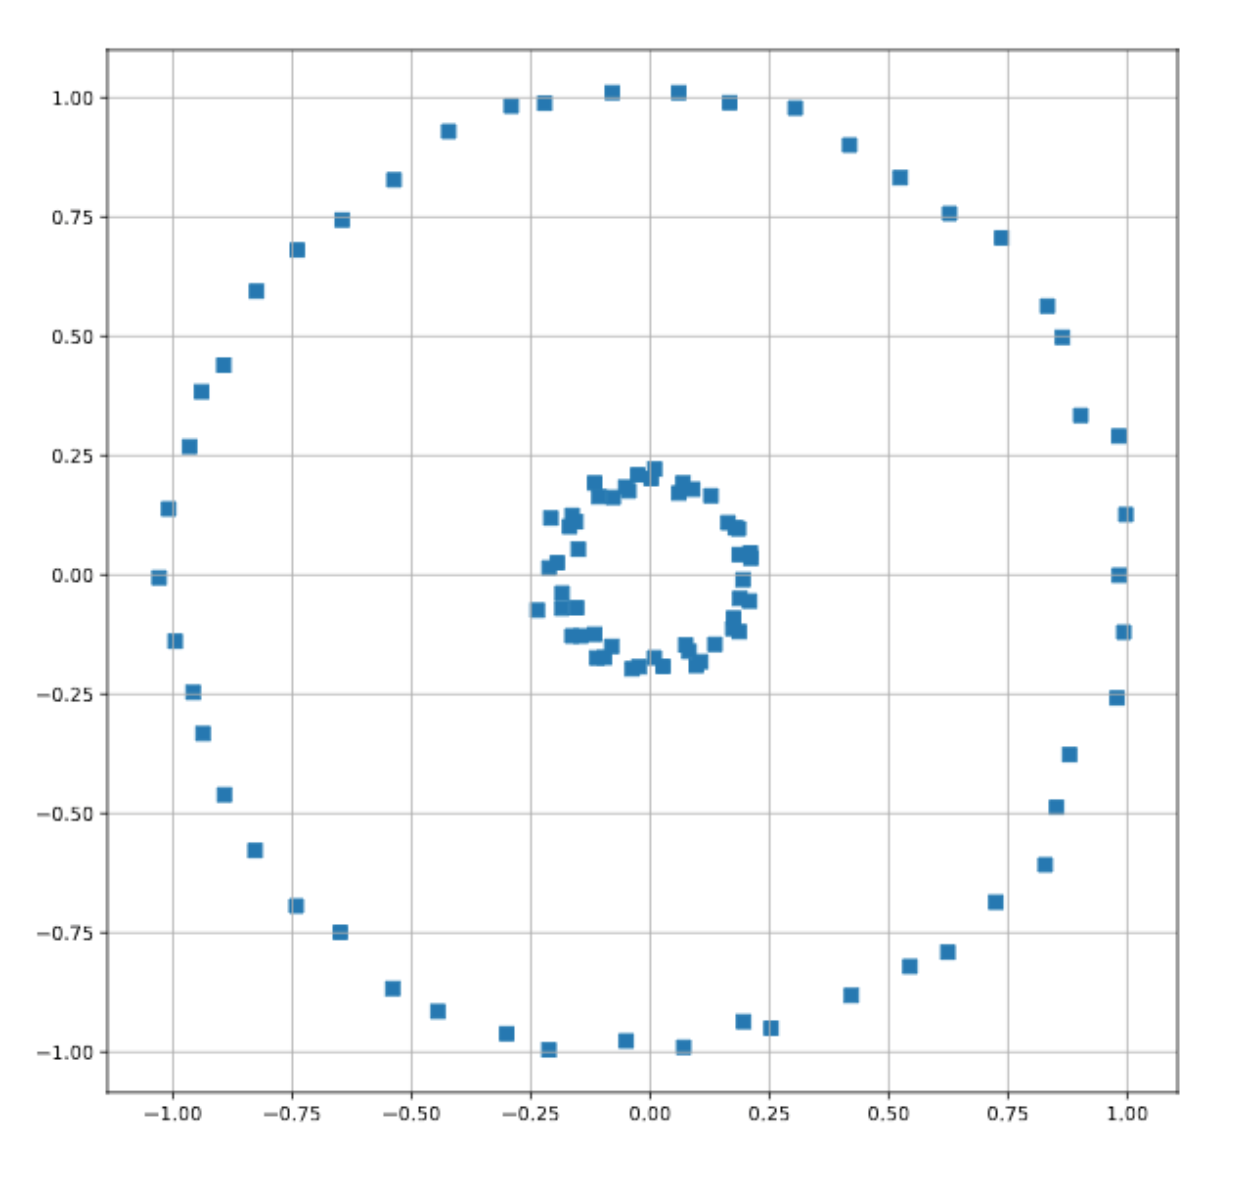
\includegraphics[scale=0.17]{circles.png}
\end{center}

\end{document}
